\scanpage{67}
passage to complements) the ten ``triangles'' of $I$, \unsure{corresponding|correspond} to the ten faces of the skew icosahedron ($\simeq$ pairs of opposite faces of the ordinary icosahedron), whereas the $15$ partitions of type $(2,2,1)$ of $I$, which one can interpret as the square structures on four of the $5$ points of $I$
\figure{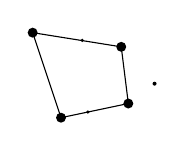
\begin{tikzpicture}[scale=.9]\draw (0,1.1)--(1.25,.9)--(1.35,.1)--(.4,-.1)--cycle;\foreach \p in {(0,1.1),(1.25,.9),(1.35,.1),(.4,-.1)}{\fill \p circle (2pt);}\fill (.7,.99) circle (.7pt);\fill (.78,-.02) circle (.7pt);\fill (1.72,.38) circle (.8pt);\end{tikzpicture}}
(by associating with such a square the two pairs of diagonally opposite vertices) correspond to the $15$ edges of the said skew icosahedron.
\margin{NB to a side $a$ one associates the set of ``colors'' of the $4$ other sides of the \deleted{\unsure{two}} adjacent faces, grouped \deleted{\unsure{two}} \unsure{into} two pairs \unsure{of the two faces}
\figure{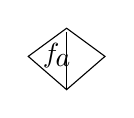
\begin{tikzpicture}[scale=.65]\draw (0,0)--(.75,.55)--(1.5,0)--(.75,-.65)--cycle;\draw (.75,.48)--(.75,-.65);\node at (.45,.02) {$f$};\node at (.68,-.08) {$a$};\end{tikzpicture}}}
A side \inserted{$a$} is contained \deleted{in}\inserted{(\uline{incident})} to a face \inserted{$f$} of the icosahedron, if and only if the ``triangle'' $\subset I$ corresponding to $f$ has as intersection with the square corresponding to $a$, \unsure{\deleted{two}\inserted{one of the}|\inserted{one of the} two} \deleted{\unsure{côt}} $2$ \deleted{consecutive}\inserted{opposite} vertices of the square, \deleted{We therefore see.}\inserted{i.e. if and only if the complement of the triangle is formed by one of the two pairs defining the square.}
\inserted{Thus we see that} the incidence relation of divisors to vertices of the structure $\widehat M_{0,I}$, corresponds \unsure{to|:} that of the faces and edges of the skew icosahedron, or by duality, to that of the \deleted{edges}\inserted{vertices} and of the \deleted{faces}\inserted{edges} of the dodecahedron.

We have therefore found:
\margin{66}
